\documentclass[tikz,border=3.14mm]{standalone}
\usepackage{amsmath}
\usepackage{amsfonts}

\begin{document}
	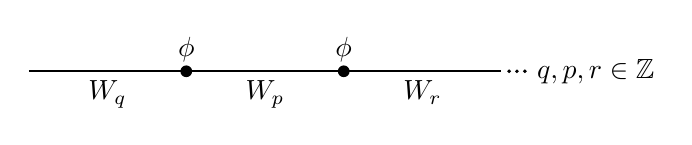
\begin{tikzpicture}[
		dot/.style={circle, fill=black, inner sep=1.5pt},
		infinity/.style={thick}
		]
		
		% Parameters
		\def\linelength{6}
		\def\dotposA{2}
		\def\dotposB{4}
		
		% Draw the main line
		\draw[thick] (0,0) -- (\linelength,0);
		
		% Draw dots at the end
		\node[circle, fill=black, inner sep=0.5pt] at (6.1,0) {};
		\node[circle, fill=black, inner sep=0.5pt] at (6.2,0) {};
		\node[circle, fill=black, inner sep=0.5pt] at (6.3,0) {};
		
		%Draw symbols at the end
		\node at (7.2,0) {$q,p,r\in\mathbb{Z}$};
	
		
		% Draw the two dots
		\node[dot] at (\dotposA,0) {};
		\node[dot] at (\dotposB,0) {};
		
		% Label the dots with phi
		\node[above] at (\dotposA,0) {$\phi$};
		\node[above] at (\dotposB,0) {$\phi$};
		
		% Add W labels
		\node[below] at (\dotposA/2,0) {$W_q$};
		\node[below] at ({\dotposA + (\dotposB-\dotposA)/2},0) {$W_p$};
		\node[below] at ({\dotposB + (\linelength-\dotposB)/2},0) {$W_r$};
		
	\end{tikzpicture}
\end{document}